\documentclass[mathserif
, handout
]{beamer}
 
 % \useoutertheme{wuerzburg}
%  \useinnertheme[outline]{chamfered}

\usepackage{tabu}
\usepackage{rotating}
\usepackage[]{algorithm2e}
\usepackage{color, colortbl}
%\usepackage{default}
\usepackage{fontspec}
\usepackage{polyglossia} 
\setmainlanguage{vietnamese}
%\setdefaultlanguage{vietnamese} 
%\setmainfont{Palatino}
 \usepackage{wasysym}
\usepackage{pifont}% http://ctan.org/pkg/pifont

\usepackage{multicol}
\usepackage{sidecap}

\usepackage{hyperref}

\usepackage{pgf}    
\usepackage{tikz}
\usetikzlibrary{arrows,automata,decorations.pathmorphing,backgrounds,positioning,fit}
\usepackage{array}
\usepackage{listings}

\usepackage{enumerate}
%\usepackage{amsmath,mathtools}
%		\usepackage{fink}

\usepackage{amsmath,amsthm, amssymb}
\usepackage{microtype}
\usetikzlibrary{arrows,automata}
\usetikzlibrary{decorations.pathmorphing}


\usetikzlibrary{calc}

 

\usetikzlibrary{trees}
\usepackage{listings}

\setbeamertemplate{footline}[frame number]
\setbeamertemplate{navigation symbols}{}%remove navigation symbols

%\usepackage{listingsutf8}

%\setbeameroption{show notes on second screen=right}


  
%\newtheorem{Lemme}{Bổ đề} 
%\newtheorem*{LI}{Lemme d'itération infinie}

%\newtheorem{Proposition}{Mệnh đề}[section]
%\newtheorem{Theorem}{Định lý}[section]
%\newtheorem{Corollaire}{Hệ quả}[section]
%\newtheorem*{Conjecture}{Giả thuyết}
% \newtheorem*{Probleme}{Bài toán}
% \newtheorem*{Fait}{Fait}
% 
% 
% \theoremstyle{definition} \newtheorem{Definition}{Định nghĩa}
% \theoremstyle{definition} \newtheorem{example}{Ví dụ}
% \theoremstyle{remark} \newtheorem*{Remarque}{Chú ý}


\usetikzlibrary{arrows,automata}



\usetikzlibrary{trees}


% \newcommand{\mnvect}[2]
% {
%   \begin{bmatrix}	#1\\#2
%   \end{bmatrix}
% }

\definecolor{olive}{rgb}{0.3, 0.4, .1}
\definecolor{fore}{RGB}{249,242,215}
\definecolor{back}{RGB}{51,51,51}
\definecolor{title}{RGB}{255,0,90}
\definecolor{dgreen}{rgb}{0.,0.7,0. }
\definecolor{gold}{rgb}{1.,0.84,0.}
\definecolor{JungleGreen}{cmyk}{0.99,0,0.52,0}
\definecolor{BlueGreen}{cmyk}{0.85,0,0.37,0}
\definecolor{RawSienna}{cmyk}{0,0.72,1,0.45}
\definecolor{Magenta}{cmyk}{0,1,0,0} 



%

%\setlength{\topmargin}{0cm} \setlength{\oddsidemargin}{0cm}
%\setlength{\evensidemargin}{0cm} \setlength{\textwidth}{17truecm}
%\setlength{\textheight}{21.0truecm}


%\parindent = 3 pt
%\parskip = 12 pt

%\newtheorem*{LI}{Lemme d'itération infinie}



\newtheorem{prprt}{Propriété}
\newtheorem{prpstn}{Mệnh đề}
\newtheorem{thrm}{Định lý}
\newtheorem{lmm}{Bổ đề}

\newtheorem{crllr}{Hệ quả}
\newtheorem{clm}{Fait}
\newtheorem{nt}{Notation}
 
\newtheorem*{cnjctr}{Conjecture}
\newtheorem{prblm}{Problème}
\newtheorem{qstn}{Question}
\newtheorem{fct}{Fait}
%\newtheorem{xmpl}{Exemple}
\newtheorem{rmrk}{Nhận xét}

\theoremstyle{example}
\newtheorem{xmpl}{Ví dụ}
\newtheorem{xrcs}{Bài tập}
  \newtheorem{dfntn}{Định nghĩa}
  

% \declaretheorem[name=Problème]{prblm}
% \declaretheorem[name=Question, style=remark, numbered=no]{qstn}

% \declaretheorem[name=Théorème, numberwithin=section]{thrm}
% \declaretheorem[name=Lemme, sibling=thrm]{lmm}
% \declaretheorem[ name=Propriété, sibling=thrm]{prprt}
% \declaretheorem[ name=Proposition, sibling=thrm]{prpstn}
% \declaretheorem[name=Corollaire, sibling=thrm]{crllr}
% \declaretheorem[name=Fait, sibling=thrm]{fct}
% \declaretheorem[name=Notation, sibling=thrm]{nt}


% \declaretheorem[style=definition, name=Définition, sibling=thrm]{dfntn}

% %\theoremstyle{definition} \newtheorem{dfntn}{Définition}[section]

% \renewcommand\thmcontinues[1]{reprise de p.\,\pageref{#1}}

% \declaretheorem[style=remark, name=Exemple%, numberwithin=section
% ]{xmpl}

% \declaretheorem[style=remark, name=Remarque, numbered=no]{rmrk}

% %\declaretheorem[style=definition,numberwithin=chapter,name = Exemple]{xmpl}

% %\theoremstyle{remark} \newtheorem{xmpl}{Exemple}[chapter]

% %\theoremstyle{remark} \newtheorem*{rmrk}{Remarque}



\newtheorem{cs}{Cas}


\def\mclose{\texttt{close}}
\def\mopen{\texttt{open}}

\def\mmclose{\texttt{\scriptsize close}}
\def\mmopen{\texttt{\scriptsize open}}



% \newcommand{\mvect}[2]
% {
% \bigl[ \begin{smallmatrix}
% #1\\ #2
% \end{smallmatrix} \bigr]
% }

% \newcommand{\mnvect}[2]
% {
%   \begin{bmatrix}	#1\\#2
%   \end{bmatrix}
% }

% % \newcommand{\mnvect}[2]
% % {
% % #1/#2
% %   % \begin{bmatrix}	#1\\#2
% %   % \end{bmatrix}
% % }

% \newcommand{\XMPL}[3]
% {
%   \begin{xmpl}
%     Soient $L=\{#1\}$ et $\Sigma=\{#2\}$. On peut vérifier que $L$ est \orl\ avec le
%     relateur de base $#3$.
%   \end{xmpl}
% }

% \newcommand{\XMP}[4]
% {
%   \begin{xmpl}[#4]
%     Soient $L=\{#1\}$ et $\Sigma=\{#2\}$. On peut vérifier que $L$ est \orl\ avec le
%     relateur de base $#3$.
%   \end{xmpl}
% }

% \newcommand{\Pui}[2]
% {
%   #1^{\leq #2}
% }


% % \newcommand{\XMPL1}[4]
% % {
% %   \begin{xmpl}
% %     Soient $L=\{#1\}$ et $\Sigma=\{#2\}$. Il est clair que $L$ est \orl\ avec le
% %     relateur de base $#3$. $L^\omega$ est un 
% %   \end{xmpl}
% % }

% \def\vvs{\vspace{11pt}}
% \def\nni{\noindent}


% \newcommand{\cas}[1]
% {
% \vvs\nni
% \textbf{Cas #1 :}
% }



% \newcommand{\souscas}[1]
% {
% \vvs\nni
% \textbf{Sous-cas #1 :}
% }

% \def\pcom{paire de mots incompatibles}
% \def\wpcom{paire de mots $\infty$-incompatible}

% \def\upcom{une paire de mots incompatibles}
% \def\uwpcom{une paire de mots $\infty$-incompatibles}
% \def\comp{\asymp}

% \def\wg{code générateur}

%  \def\gc{code générateur}

% \def\gcx{codes générateurs}
% \def\Gcx{Codes générateurs }
% \def\ugc{un code générateur}
% \def\Ugc{un Code générateur}

% \def\wgc{$\omega$-code générateur}
% \def\wgcx{$\omega$-codes générateurs}
% \def\wGcx{$\omega$-Codes générateurs }
% \def\wugc{un $\omega$-code générateur}
% \def\wUgc{un $\omega$-code générateur}

% \def\orl {langage à un relateur}

% \def\orlx {langages à un relateur}
% \def\Orlx {Langages à un relateur}
% \def\uorl {un langage à un relateur}


% \def\ugc{un code générateur}

% \def\cp{code préfixe}

% \def\iff{si et seulement si} 
% \def\w{\omega}

% \def\CODE{la proposition~\ref{c3prop23}, $L^\omega$ n'a pas de \gc}
% \def\NOCODE{$L^\omega$ n'a pas de \gc}


\def\vs{}
\def\ni{}





%\setlength{\topmargin}{0cm} \setlength{\oddsidemargin}{0cm}
%\setlength{\evensidemargin}{0cm} \setlength{\textwidth}{17truecm}
%\setlength{\textheight}{21.0truecm}


%\parindent = 3 pt
%\parskip = 12 pt

%\newtheorem*{LI}{Lemme d'itération infinie}



\newtheorem{prprt}{Propriété}
\newtheorem{prpstn}{Mệnh đề}
\newtheorem{thrm}{Định lý}
\newtheorem{lmm}{Bổ đề}
\newtheorem{rl}{Luật}

\newtheorem{crllr}{Hệ quả}
\newtheorem{clm}{Khẳng định}
\newtheorem{nt}{Notation}
 
\newtheorem*{cnjctr}{Giả thuyết}

\newtheorem{fct}{Fait}
%\newtheorem{xmpl}{Exemple}

\theoremstyle{example}
\newtheorem{xmpl}{Ví dụ}
\newtheorem{xrcs}{Bài tập}
  \newtheorem{dfntn}{Định nghĩa}
  \newtheorem{qstn}{Câu hỏi}
\newtheorem{prblm}{Bài toán}  
   \newtheorem{sol}{Lời giải}
\newtheorem{rmrk}{Nhận xét}
  
%  \newtheorem{rmrk}{Định nghĩa}
  

% \declaretheorem[name=Problème]{prblm}
% \declaretheorem[name=Question, style=remark, numbered=no]{qstn}

% \declaretheorem[name=Théorème, numberwithin=section]{thrm}
% \declaretheorem[name=Lemme, sibling=thrm]{lmm}
% \declaretheorem[ name=Propriété, sibling=thrm]{prprt}
% \declaretheorem[ name=Proposition, sibling=thrm]{prpstn}
% \declaretheorem[name=Corollaire, sibling=thrm]{crllr}
% \declaretheorem[name=Fait, sibling=thrm]{fct}
% \declaretheorem[name=Notation, sibling=thrm]{nt}


% \declaretheorem[style=definition, name=Définition, sibling=thrm]{dfntn}

% %\theoremstyle{definition} \newtheorem{dfntn}{Définition}[section]

% \renewcommand\thmcontinues[1]{reprise de p.\,\pageref{#1}}

% \declaretheorem[style=remark, name=Exemple%, numberwithin=section
% ]{xmpl}

% \declaretheorem[style=remark, name=Remarque, numbered=no]{rmrk}

% %\declaretheorem[style=definition,numberwithin=chapter,name = Exemple]{xmpl}

% %\theoremstyle{remark} \newtheorem{xmpl}{Exemple}[chapter]

% %\theoremstyle{remark} \newtheorem*{rmrk}{Remarque}



\newtheorem{cs}{Cas}


\def\mclose{\texttt{close}}
\def\mopen{\texttt{open}}

\def\mmclose{\texttt{\scriptsize close}}
\def\mmopen{\texttt{\scriptsize open}}



% \newcommand{\mvect}[2]
% {
% \bigl[ \begin{smallmatrix}
% #1\\ #2
% \end{smallmatrix} \bigr]
% }

% \newcommand{\mnvect}[2]
% {
%   \begin{bmatrix}	#1\\#2
%   \end{bmatrix}
% }

% % \newcommand{\mnvect}[2]
% % {
% % #1/#2
% %   % \begin{bmatrix}	#1\\#2
% %   % \end{bmatrix}
% % }

% \newcommand{\XMPL}[3]
% {
%   \begin{xmpl}
%     Soient $L=\{#1\}$ et $\Sigma=\{#2\}$. On peut vérifier que $L$ est \orl\ avec le
%     relateur de base $#3$.
%   \end{xmpl}
% }

% \newcommand{\XMP}[4]
% {
%   \begin{xmpl}[#4]
%     Soient $L=\{#1\}$ et $\Sigma=\{#2\}$. On peut vérifier que $L$ est \orl\ avec le
%     relateur de base $#3$.
%   \end{xmpl}
% }

% \newcommand{\Pui}[2]
% {
%   #1^{\leq #2}
% }


% % \newcommand{\XMPL1}[4]
% % {
% %   \begin{xmpl}
% %     Soient $L=\{#1\}$ et $\Sigma=\{#2\}$. Il est clair que $L$ est \orl\ avec le
% %     relateur de base $#3$. $L^\omega$ est un 
% %   \end{xmpl}
% % }

% \def\vvs{\vspace{11pt}}
% \def\nni{\noindent}


% \newcommand{\cas}[1]
% {
% \vvs\nni
% \textbf{Cas #1 :}
% }



% \newcommand{\souscas}[1]
% {
% \vvs\nni
% \textbf{Sous-cas #1 :}
% }

% \def\pcom{paire de mots incompatibles}
% \def\wpcom{paire de mots $\infty$-incompatible}

% \def\upcom{une paire de mots incompatibles}
% \def\uwpcom{une paire de mots $\infty$-incompatibles}
% \def\comp{\asymp}

% \def\wg{code générateur}

%  \def\gc{code générateur}

% \def\gcx{codes générateurs}
% \def\Gcx{Codes générateurs }
% \def\ugc{un code générateur}
% \def\Ugc{un Code générateur}

% \def\wgc{$\omega$-code générateur}
% \def\wgcx{$\omega$-codes générateurs}
% \def\wGcx{$\omega$-Codes générateurs }
% \def\wugc{un $\omega$-code générateur}
% \def\wUgc{un $\omega$-code générateur}

% \def\orl {langage à un relateur}

% \def\orlx {langages à un relateur}
% \def\Orlx {Langages à un relateur}
% \def\uorl {un langage à un relateur}


% \def\ugc{un code générateur}

% \def\cp{code préfixe}

% \def\iff{si et seulement si} 
% \def\w{\omega}

% \def\CODE{la proposition~\ref{c3prop23}, $L^\omega$ n'a pas de \gc}
% \def\NOCODE{$L^\omega$ n'a pas de \gc}


\def\vs{}
\def\ni{}


\def\trail{hành trình đơn}
\def\Trail{Hành trình đơn}

\def\ctrail{\trail\ đóng}
\def\Ctrail{\Trail\ đóng }

\def\walk{hành trình}
\def\Walk{Hành trình}

\def\cwalk{hành trình đóng}
\def\Cwalk{Hành trình đóng}

\def\path{đường đi}
\def\Path{Đường đi}
 
\def\conn{liên thông}
\def\Conn{Liên thông}

\def\Comp{Thành phần liên thông}
\def\comp{thành phần liên thông}

\def\Cuted{Cạnh cắt}
\def\cuted{cạnh cắt}

\def\Cutve{Đỉnh cắt}
\def\cutve{đỉnh cắt}

\def\Induced{Đồ thị con cảm sinh}
\def\induced{đồ thị con cảm sinh}

 
\def\iff{{\color{blue} nếu và chỉ nếu}}

\def\ideg{\text{indeg}}
\def\odeg{\text{outdeg}}

\def\pr{\mathrm{Pr}}
\def\ex{\mathrm{Ex}}
\def\S{\mathcal{S}}
\def\var{\mathrm{Var}}

\def\F{\mathbb{F}}
\def\Z{\mathbb{Z}}
\def\N{\mathbb{N}}
\def\ord{\mathrm{ord}}
\newcommand{\bigO}{\ensuremath{\mathcal{O}}}% big-O notation/symbol


 \newcommand{\defi}[1]{{\color{blue}{\textbf{\emph{#1}}}}}
\newcommand{\contradiction}{{\hbox{%
    \setbox0=\hbox{$\mkern-3mu\times\mkern-3mu$}%
    \setbox1=\hbox to0pt{\hss$\times$\hss}%
    \copy0\raisebox{0.5\wd0}{\copy1}\raisebox{-0.5\wd0}{\box1}\box0
}}}

\newcommand{\cmark}{{\color{blue}\Large\ding{51}}}%
\newcommand{\xmark}{{\color{red}\Large\ding{55}}}%

%\newcommand{\defi}[1]{{\color{blue}{\textbf{\emph{#1}}}}}


 \AtBeginSection[]  
 { 
   \begin{frame}[plain]{Nội dung} 
     \tableofcontents[currentsection,currentsubsection] 
   \end{frame} 
 }  



\begin{document}
% \tikzstyle{every picture}+=[remember picture]

% \tikzstyle{na} = [baseline=-.5ex]

\author{Trần Vĩnh Đức}
%\institute[HUST]{Hanoi University of Science and Technology}

  
% \newcommand{\cmark}{{\color{blue}\Large\ding{51}}}%
% \newcommand{\xmark}{{\color{red}\Large\ding{55}}}%
\title{Logarit rời rạc} 
 \author{Toán Chuyên Đề}   
\institute[HUST]{HUST} 
   
\maketitle      

\begin{frame}{Tài liệu tham khảo}
  \begin{itemize}
  \item J. Hoffstein, J. Pipher, J. H. Silverman,
    \textit{An Introduction to Mathematical Cryptography},
    Springer-Verlag – Undergraduate Texts in Mathematics, 2nd Ed.,
    2014.
  \item T. H. Cormen, C. E. Leiserson, R. L. Rivest, C. Stein.  \textit{Introduction to Algorithms}, Third Edition (3rd ed.). The MIT Press. 2009.

  \item H. H. Khoái, P. H. Điển, \textit{Số học thuật toán: cơ sở lý thuyết và tính toán thực hành}, NXB Đại học Quốc gia Hà Nội, 2003.
  \end{itemize}
%  \item Phan .Đ. Diệu, \textit{Logic toán \& cơ sở toán học}. (2003)  
\end{frame}

\section{Bài toán Logarit rời rạc}
\begin{frame}{Nhắc lại}
  \begin{itemize}
  \item Xét số nguyên tố (lớn) $p$  và trường hữu hạn  $\F_p$.
  \item Tồn tại căn nguyên thủy $g$, tức là mọi phần tử khác $0$ của $\F_p$ đều là một lũy thức nào đó của $g$.
  \item Cụ thể 
    $$
    g^{p-1} = 1.
    $$
  \item Và 
    $$
    1,\ g,\ g^2,\ g^3,\ \cdots,\ g^{p-2} \in \F_p^*. 
    $$
  \end{itemize}
\end{frame}

\begin{frame}
  \begin{dfntn}
    Xét $g$ là một căn nguyên thủy của $\F_p$ và $h$ là một phần tử khác $0$ của $\F_p$. Bài toán Logarit rời rạc (DLP) là bài toán tìm một số mũ $x$ thỏa mãn 
    $$
    g^x \equiv h \pmod{p}.
    $$
Số $x$ được gọi là logarit rời rạc cơ sở  $g$ của $h$ và ký hiệu $\log_g(h)$. 
  \end{dfntn}
\end{frame}

\begin{frame}
  \begin{xrcs}
    Hãy tính các logarit rời rạc sau.
    \begin{enumerate}
    \item $\log_2(13)$ cho số nguyên tố $23$, cụ thể $p=23, g=2$ và bạn phải giải phương trình đồng dư $2^x\equiv 13\pmod{23}$.
    \item $\log_{10}(22)$ cho số nguyên tố $p = 47$.
    \item $\log_{627}(608)$ cho số nguyên tố $p =941$.
    \end{enumerate}
  \end{xrcs}
\end{frame}
\begin{frame}
  \begin{xmpl}
    \begin{itemize}
    \item<+-> Xét số nguyên tố $p = 56509$, và ta có thể kiểm tra $g=2$ là
      một căn nguyên thủy modun $p$. 
    \item<+-> Làm thế nào để tính
      $\log_2(38679)$?  
    \item<+-> Một phương pháp là tính
    $$
    2^0,\ 2^1,\ 2^2,\ 2^3,\ \cdots\ \pmod{56509}
    $$
    cho đến khi được lũy thừa bằng $38679$. 
  \item<+-> Bạn có thể kiểm tra rằng
    $$
    2^{11235} \equiv 38679 \pmod{56509}.
    $$
  \end{itemize}
  \end{xmpl}
\end{frame}
\begin{frame}
  \begin{rmrk}
    Nếu bài toán Logarit rời rạc có nghiệm, vậy nó có vố số nghiệm vì 
    \begin{align*}
    g^{x + k(p-1)} &= g^x\cdot g^{k(p-1)}\\      
                &=h \cdot 1^k  \qquad \qquad\qquad   \text{(Định lý Fermat)}\\
                &\equiv h \pmod{p}. 
    \end{align*}
  \end{rmrk}
\end{frame}

\begin{frame}
  \begin{xrcs}
    Chứng minh rằng $\log_g$ là một hàm 
    $$
    \log_g : \F_p^* \longrightarrow \Z/(p-1)\Z.
    $$
  \end{xrcs}
\end{frame}
\begin{frame}
  \begin{xrcs}
    Chứng minh rằng 
    $$
    \log_g(ab) = \log_g(a) + \log_g(b).
    $$
  \end{xrcs}
\end{frame}

\begin{frame}
  \begin{rmrk}
    Bài toán logarit rời rạc không cần phải giả sử cơ sở $g$ là một phần tử sinh của $\F_p$. Nói chung, xét $g \in \F_p^*$ và $h \in \F_p^*$, bài toán logarit rời rạc là xác định $x$ sao cho $g^x \equiv h \pmod{p}$, giả sử rằng $x$ tồn tại. 
  \end{rmrk}
\end{frame}

\begin{frame}{Tính  ngẫu nhiên của lũy thừa $627^i \pmod{941}$}
  \begin{block}{}
    \centering
    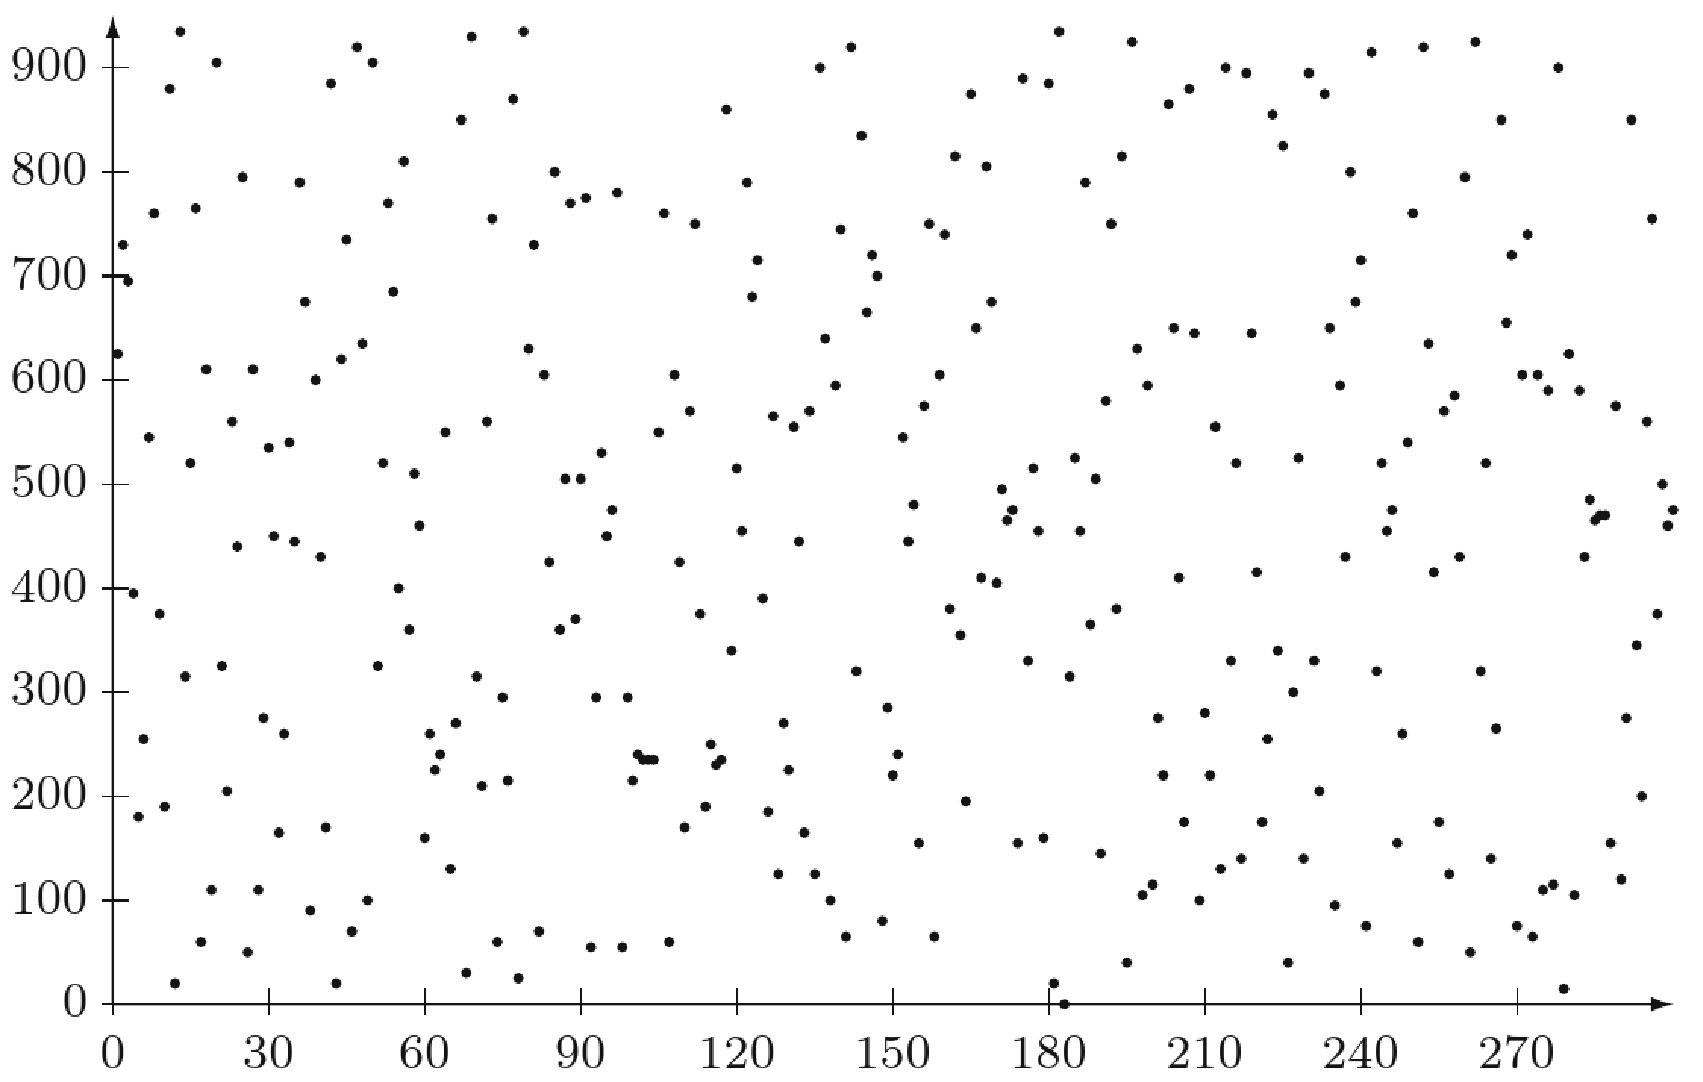
\includegraphics[width=0.9\textwidth]{fig22.pdf}
  \end{block}
\end{frame}

\begin{frame}{Bài toán logarit rời rạc trong nhóm}
  \begin{dfntn}
Xét nhóm $G$ với phép toán $\star$. Bài toán Logarit rời rạc cho $G$ là xác định số nguyên $x$ thỏa mãn 
$$
\underbrace{g\star g\star \cdots \star g}_{x \text{ lần }} = h 
$$
với hai phần tử $h$ và $g$ trong $G$ cho trước.
  \end{dfntn}
\end{frame}

\section{Phương pháp trao đổi khóa Diffie-Hellman}

\begin{frame}{Bài toán}
  \begin{itemize}
  \item Alice và Bob muốn trao đổi một khóa $k$ chung dùng để mã hóa thông tin.
  \item Nhưng họ chỉ có một kênh trao đổi không an toàn: Thông tin truyền có thể  bị nghe trộm. 
  \item Liệu có cách để Alice và Bob trao đổi khóa mà dù bị Eve có nghe trộm?
  \end{itemize}
\end{frame}

\begin{frame}{Giao thức Diffie-Hellman}
  \begin{itemize}
  \item Alice và Bob thống nhất một số nguyên tố (lớn) $p$ và một số nguyên $g \pmod{p}$.
  \item Tốt nhất họ nên chọn $g$ sao cho cấp của $g$ trong $\F_p^*$ là một số nguyên tố lớn.
  \item Alice và Bob để hai giá trị $p$ và $g$ công khai (trên Website của của họ).
  \end{itemize}
  \begin{block}{}
    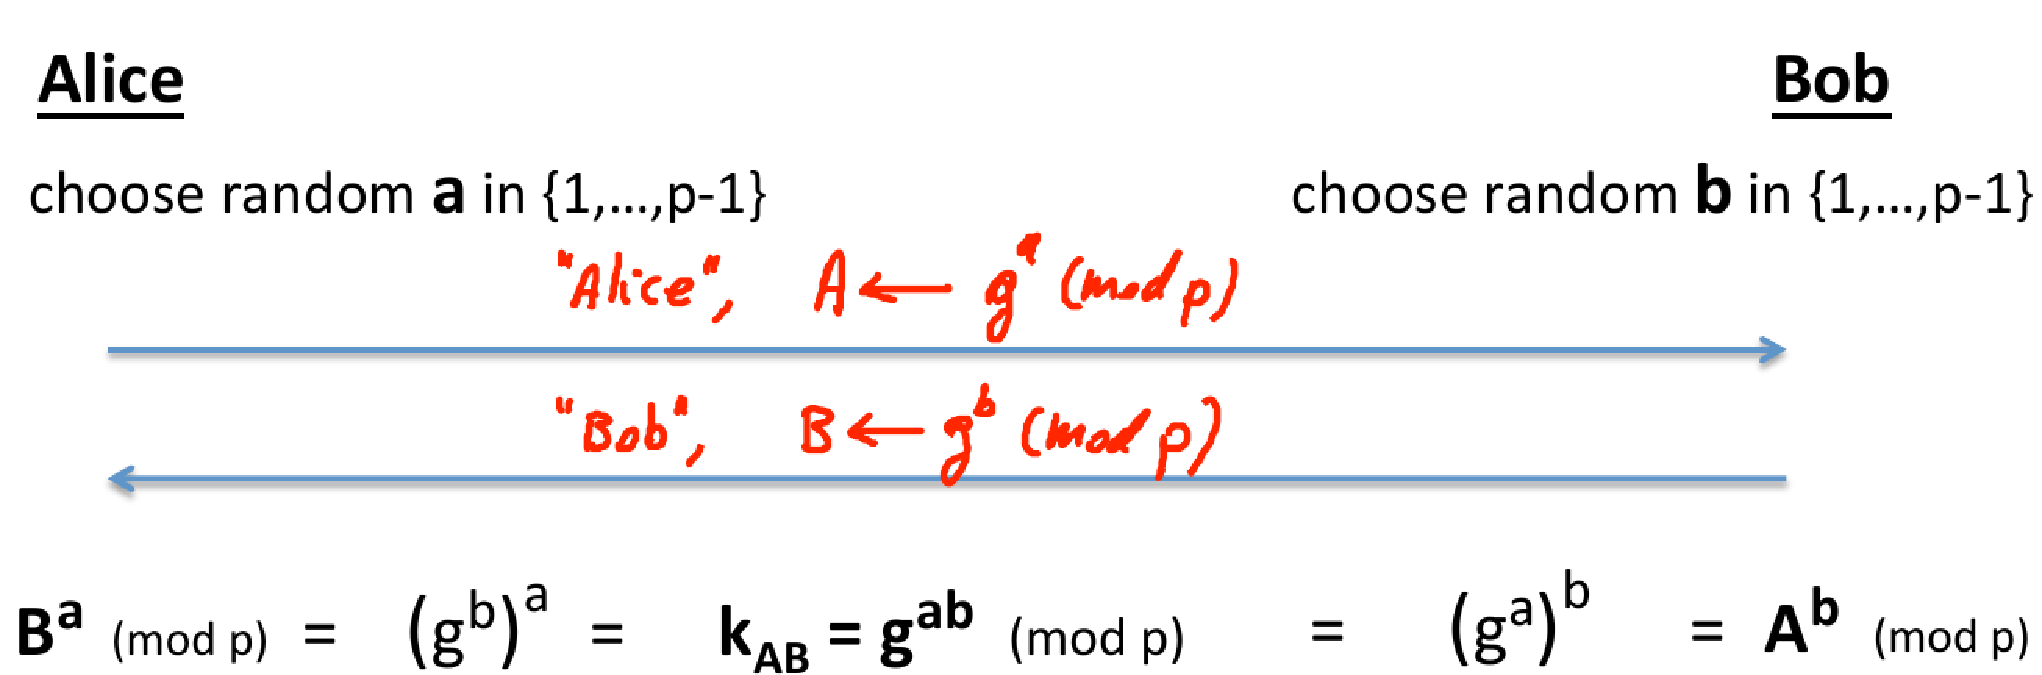
\includegraphics[width=\textwidth]{DH.pdf}
  \end{block}
\end{frame}
\begin{frame}
  \begin{xmpl}
    \begin{itemize}
    \item Alice và Bob thống nhất sử dụng số $p=941$ và căn nguyên thủy $g = 627$.
    \item Alice chọn khóa bí mật $a = 347$.
    \item Bob chọn khóa bí mật $b = 781$.
    \item Hãy tính giá trị khóa chia sẻ của Alice và Bob.
    \end{itemize}
  \end{xmpl}
\end{frame}

\begin{frame}
  \begin{dfntn}
    Xét $p$ là một số nguyên tố và $g$ là một số nguyên. Bài toán \alert{Diffie-Hellman} (DHP) là bài toán tính giá trị của 
    $$
    g^{ab}\pmod{p}
    $$
    từ các giá trị $g^a\pmod{p}$ và $g^b\pmod{p}$.
  \end{dfntn}
\end{frame}

\begin{frame}{DLP  chọi DHP }
  \begin{xrcs}
    Hãy chứng minh rằng DHP  không khó hơn DLP.  Có nghĩa rằng, nếu ta có thuật toán hiệu quả giải DLP, thì ta cũng có thuật toán hiệu quả giải DHP.
  \end{xrcs}\pause 
  \begin{rmrk}
    Ngược lại, giả sử rằng Eve có thuật toán hiệu quả giải DHP. Liệu cô ta có thể giải bài toán DLP? Đây vẫn là câu hỏi mở.
  \end{rmrk}
\end{frame}
\begin{frame}
  \begin{xrcs}
    \begin{itemize}
    \item<+-> Alice và Bob dùng số nguyên tố $p = 1373$ và cơ sở $g=2$ để
      trao đổi khóa. 
    \item<+-> Alice gửi Bob giá trị $A=974$.
    \item<+-> Bob chọn số bí mật $b = 871$.
    \item<+-> Bob nên gửi cho Alice giá trị gì, và khóa bí mật họ chia sẻ là gì?
    \item<+-> Bạn có thể đoán được số bí mật $a$ của Alice?
    \end{itemize}
  \end{xrcs}
\end{frame}

\section{Sơ lược về lý thuyết nhóm}
\begin{frame}{Một số tính chất của $\F_p^*$}
	\begin{itemize}
		\item<+-> Có phần tử $1 \in \F_p^*$ thỏa mãn $1 \cdot a =  a$.
		\item<+-> Mọi phần tử $a \in \F_p^*$ đều có phần tử nghịch đảo $a^{-1}$ thỏa mãn $a\cdot a^{-1} = 1$.
		\item<+-> Phép nhân có tính chất kết hợp: $a \cdot (b\cdot c) = (a \cdot b)\cdot c $.
		\item<+-> Phép nhân có tính chất giao hoán: $a \cdot b = b \cdot a$.   
	\end{itemize}
\end{frame}
%--- Next Frame ---%

\begin{frame}{Tính chất của $\F_p^*$ liên quan đến phép cộng}
	\begin{itemize}
		\item<+-> Có phần tử $0 \in \F_p^*$ thỏa mãn $0 +  a =  a$.
		\item<+-> Mọi phần tử $a \in \F_p^*$ đều có phần tử nghịch đảo $-a$ thỏa mãn $a + (-a) = 0$.
		\item<+-> Phép cộng có tính chất kết hợp: $a + (b + c) = (a + b)+ c $.
		\item<+-> Phép cộng có tính chất giao hoán: $a + b = b + a$.   
	\end{itemize}
\end{frame}
%--- Next Frame ---%

\begin{frame}
	\begin{dfntn}
		Một nhóm bao gồm một tập $G$ và một phép toán hai ngôi $\star$ trên $G$ thỏa mãn ba tính chất:
		\begin{description}
			\item<+->[ Có đơn vị: ] Tồn tại một phần tử $e \in G$ sao cho $$e\star a = a\star e = a\ \text{ với mọi } a \in G.$$
			
			\item<+->[ Có nghịch đảo: ] Với mỗi phần tử $a \in G$ tồn tại $a^{-1} \in G$ sao cho
			$$
			a \star a^{-1} = a^{-1} \star a = 1.
			$$ 
			\item<+->[ Kết hợp:  ] $a\star (b\star c) = (a\star b)\star c$,\ $\text{ với mọi } a,b,c \in G$.
		\end{description}
	\end{dfntn}
\end{frame}
%--- Next Frame ---%

\begin{frame}
	\begin{dfntn}
		Nhóm $G$ với phép toán $\star$ có  tính chất 
		\begin{description}
			\item<+->[ Giao hoán: ] $a \star b = b \star a$\  với mọi  $a,b \in G$,
		\end{description}
		được gọi là nhóm giao hoán hoặc nhóm Abel.
	\end{dfntn}
\end{frame}
%--- Next Frame ---%

\begin{frame}
	\begin{dfntn}
		\begin{itemize}
			\item<+-> Nếu nhóm $G$ có hữu hạn phần tử, ta gọi $G$ là nhóm hữu hạn. 
			\item<+-> Cấp của nhóm $G$ là số phần tử của $G$; nó thường được ký hiệu bởi $|G|$ hoặc $\#G$.
		\end{itemize}
	\end{dfntn}
\end{frame}
%--- Next Frame ---%

\begin{frame}
	\begin{xmpl}
		\begin{itemize}
			\item<+-> $G=F_p^*$ và $\star=$ phép nhân. Phần tử đơn vị là $e=1$. Cấp của nhóm này là gì?
			\item<+-> $G=\Z/N\Z$ và  $\star=$ phép cộng. Phần tử đơn vị là gì? Cấp của nhóm này là gì?
			\item<+-> $G = \Z$ và  $\star=$ phép cộng. Phần tử đơn vị của nhóm này là gì?  phần tử nghịch đảo của phần tử $a$ là gì? 
			\item<+-> $G = \Z$ và $\star=$ phép nhân có phải là nhóm không? Tại sao?
			\item<+-> $G = \mathbb{R}^*$ và $\star=$ phép nhân có phải là nhóm không? Tại sao?
		\end{itemize}
	\end{xmpl}
	
\end{frame}
%--- Next Frame ---%

\begin{frame}
	\begin{xrcs}
		\begin{itemize}
			\item<+-> Một ví dụ của nhóm không giao hoán là 
			$$
			G = \left\{ \begin{pmatrix}
				a & b\\
				c & d
			\end{pmatrix}\ :\ a,b,c,d \in \mathbb{R} \text{ và } ad - bc \not= 0 \right\}
			$$
			với $\star =$ phép nhân ma trận. 
			\item<+-> Phần tử đơn vị của nhóm này là gì? Hãy tìm công thức tính phần tử nghịch đảo 
			$$
			\begin{pmatrix}
							a & b\\
							c & d
						\end{pmatrix}^{-1}.
			$$
			
			\item<+-> Tại sao đây không phải là nhóm giao hoán?
		\end{itemize}
	\end{xrcs}
\end{frame}
%--- Next Frame ---%

\begin{frame}
	\begin{xmpl} Nhóm tuyến tính tổng quát 
			$$
			GL_n(\mathbb{R}) = \left\{ \text{ ma trận thực $A$ kích thước $n\times n$ với $\det(A)\not= 0$ } \right\}
			$$
			với $\star =$ phép nhân ma trận. \\
			
			\vspace{0.5cm}
			 Thay $\mathbb{R}$ bởi trường hữu hạn $\F_p^*$, ta được nhóm $GL(\F_p^*)$.
			
			
	\end{xmpl}
\end{frame}
%--- Next Frame ---%

\begin{frame}
	\begin{dfntn}
		Xét $G$ là một nhóm và $x$ là một số nguyên dương. Ta ký hiệu $g^x$ là 
		$$
		g^x = \underbrace{g\star g\star \cdots \star g}_{x \text{ lần }}
		$$
	\end{dfntn}
\end{frame}
%--- Next Frame ---%

\begin{frame}
	\begin{xmpl}
		\begin{itemize}
			\item<+-> $g^x$ trong nhóm $\mathbb{F}_p^*$ theo nghĩa thông thường.
			\item<+-> $g^x$ trong nhóm $\Z/N\Z$ với phép cộng có nghĩa rằng $$x \cdot g = g+g+\cdots +g$$ 
		\end{itemize}
	\end{xmpl}
\end{frame}


\begin{frame}
	\begin{dfntn}
		Xét nhóm $G$ và một phần tử $a\in G$. Giả sử rằng có tồn tại số nguyên dương $d$ sao cho $a^d = e$. Số nguyên nhỏ nhất $d$ có tính chất này gọi là cấp của $a$. Nếu không tồn tại số nguyên như vậy thì $a$ gọi là có cấp vô hạn. 
	\end{dfntn}
\end{frame}
%--- Next Frame ---%

\begin{frame}
	\begin{prpstn}
		\begin{itemize}
			\item<+-> 	Xét nhóm hữu hạn $G$. Vậy thì mọi phần tử của $G$ có cấp hữu hạn. 
			\item<+-> Hơn nữa, nếu $a\in G$ có cấp $d$ và nếu $a^k = e$, vậy thì $d\mid k$.

		\end{itemize}
	\end{prpstn}
	Bài tập: Hãy chứng minh mệnh đề trên.
\end{frame}
%--- Next Frame ---%

\begin{frame}
	\begin{thrm}[Lagrange] 
		\begin{itemize}
			\item<+-> Xét $G$ là nhóm hữu hạn và xét $a \in G$. Vậy thì cấp của $G$ chia hết cho cấp của $a$.
		
		
		\item<+-> Chính xác hơn, xét $n = \#G$ và $d$ là cấp của $a$, tức $a^d$ là lũy thừa nguyên dương nhỏ nhất bằng với $e$. Khi đó 
		$$
		a^n= e\qquad \text{và}\qquad d \mid n.
		$$
		\end{itemize}
		
	\end{thrm}
	Bài tập: Hãy chứng minh định lý trên.
\end{frame}
%--- Next Frame ---%

\section{Thuật toán đụng độ cho DLP}
\begin{frame}{Bài toán logarit rời rạc trong nhóm}
  \begin{dfntn}[Nhắc lại]
Xét nhóm $G$ với phép toán $\star$. Bài toán Logarit rời rạc cho $G$ là tìm số nguyên $x$ thỏa mãn
$$
g^x = h
$$
với hai phần tử $h$ và $g$ trong $G$ cho trước.
  \end{dfntn}
\end{frame}

\begin{frame}
	\begin{prpstn}[Chặn tầm thường cho DLP] Xét nhóm $G$ và $g\in G$ là một phần tử có cấp $N$. Vậy thì bài toán logarit rời rạc 
		$$
		g^x = h
		$$
		có thể được giải trong thời gian $\bigO(N)$ bước, mỗi bước gồm phép nhân với $g$.
	\end{prpstn}
\end{frame}
%--- Next Frame ---%



%--- Next Frame ---%
\begin{frame}
	\begin{prpstn}[Thuật toán Babystep-Giantstep]
		Xét nhóm $G$ và $g \in G$ là một phần tử có cấp $N \geq 2$. Thuật toán sau đây giải bài toán logarit rời rạc $g^x = h$ trong $\bigO(\sqrt{N}\cdot \log N)$ bước.
		\begin{enumerate}
			\item<+-> Đặt $n = 1 + \lfloor \sqrt{N}\rfloor$, cụ thể $n > \sqrt{N}$.
			\item<+-> Xây dựng hai danh sách:\\
			$L_1$:\qquad  $e,\ g,\ g^2,\ g^3,\ \cdots\ ,\  g^n$,\\
			$L_2$:\qquad  $h,\ h\cdot g^{-n},\  h\cdot g^{-2n},\ h\cdot g^{-3n},\ \cdots,\ h\cdot g^{-n^2}$.
			\item<+-> Tìm $i,j$ thỏa mãn $g^i = h\cdot g^{-jn}$.
			\item<+-> Vậy thì $x = i + jn$ là một nghiệm của $g^x =h$.  
		\end{enumerate}
	\end{prpstn}
\end{frame}
%--- Next Frame ---%

\begin{frame}[t]{Thuật toán Babystep-Giantstep (chi tiết)}
\begin{itemize}
	\item \emph{Input:} Các phần tử $g,h \in G$; cấp $N$ của $g$.
	\item \emph{Output: } $x = \log_g(h)$. 
\end{itemize}	
\begin{block}{}
\qquad $n = 1+\lfloor \sqrt{N}\rfloor$\\
\qquad \textbf{for } $i = 0$ to $n$ :\\
\qquad \qquad Tính $g_i = g^{i}$\\
\qquad Sắp xếp các cặp $(i,g_i)$ theo giá trị $g_i$\\
\qquad \textbf{for } $j = 0$ to $n$ :\\
\qquad \qquad Tính $h_j = h\cdot g^{-jn}$\\
\qquad \qquad \textbf{if $h_j==g_i$} với $i$ nào đó :\qquad   {\color{green}//Dùng tìm kiếm nhị phân} \\
\qquad \qquad \qquad  \textbf{return} $x = i +jn$\\
\qquad \textbf{return} "không tồn tại $x$"	
\end{block}
\end{frame}

%--- Next Frame ---%
\begin{frame}{Bài tập}
	\begin{itemize}
		\item<+-> Xét nhóm $\F_{29}^*$ có cấp $N = 29-1=28$.
		\item<+-> Lấy $g=2$ và $h = 17$.
		\item<+-> Ta có $n = 6.$
		\item<+-> Ta đã tính các lũy thừa $g^i$ như bảng dưới đây. Hãy hoàn thành nốt bảng và tìm $\log_2(17)$:
$$		\begin{tabu}{c|ccccccc}
		i &0  &1  &2  &3  &4  &5  &6\\
		\hline 
		 g^i &1  &2  &4  &8  &16  &3  &6\\
		 h\cdot g^{-6i}
		\end{tabu} 	  
$$	
biết rằng $2^{-6} = 5$.
\end{itemize}
\end{frame}
%--- Next Frame ---%

\section{Định lý phần dư Trung Hoa}
\begin{frame}{Bài toán}
	\begin{itemize}
		\item<+-> Có một số vật ta chưa biết số lượng bao nhiêu.
		\item<+-> Số này chia $3$ dư $2$.
		\item<+-> Số này chia $5$ dư $3$.
		\item<+-> Số này chia $7$ dư $2$.
		\item<+-> Hỏi có bao nhiêu vật ?    
	\end{itemize}
\end{frame}
%--- Next Frame ---%

\begin{frame}%{Hệ phương trình đồng dư}
	\begin{xmpl}
		Tìm số nguyên $x$ thỏa mãn đồng thời cả hai phương trình
		\[
			x \equiv 1 \pmod{5} \qquad \text{và} \qquad x\equiv 9 \pmod{11}.
		\]
Nghiệm của phương trình thứ nhất là tập các số nguyên 
\[
	x = 1 + 5y,\qquad y \in \Z.
\]
Thế vào phương trình thứ hai, ta được 
\[
1 + 5y \equiv 9\pmod{11}\qquad  \Leftrightarrow\qquad  5y \equiv 8\pmod{11}  
\]
Nhân cả hai vế với $5^{-1} \equiv 9 \pmod{11}$. Ta được $$y \equiv 9\cdot 8 \equiv 72 \equiv 6 \pmod{11} $$ 
Thay lại vào phương trình đầu ta được 
$
x = 1 + 5 \cdot 6 = 31.
$
	\end{xmpl}	
\end{frame}

\begin{frame}
	\begin{thrm}[Định lý phần dư Trung Hoa]
		Xét $m_1, m_2, \dots, m_k$ là các số đôi một nguyên tố cùng nhau. Xét các số nguyên $a_1, a_2, \dots, a_k$ bất kỳ. Khi đó hệ phương trình
		\[
		x \equiv a_1\pmod{m_1},\quad x \equiv a_2\pmod{m_2},\quad \cdots,\quad x \equiv a_k\pmod{m_k} 
		\]
		có một nghiệm $x = c$. Hơn nữa, nếu $x=c$ và $x=c'$ là hai nghiệm của hệ, vậy thì 
		$$
			c \equiv c'  \pmod{m_1 m_2 \dots m_k}.
		$$
	\end{thrm}
\end{frame}
%--- Next Frame ---%

\begin{frame}
	\begin{xmpl}
\begin{itemize}
	\item<+-> Xét hệ ba phương trình sau đây 
		\[
			x \equiv 2 \pmod{3},\qquad x\equiv 3 \pmod{7},\qquad x \equiv 4 \pmod{16}. 
		\]
		
		\item<+-> Dùng một nghiệm $x=2$ của phương trình đầu để tìm nghiệm thỏa mãn cả hai phương trình đầu tiên. Ta được $x = 17$.
 
 \item<+-> Dùng nghiệm này để tìm nghiệm thỏa mãn cả ba phương trình. Ta được $x=164$. 
\end{itemize}			
\end{xmpl}
\end{frame}
%--- Next Frame ---%

\begin{frame}{Công thức nghiệm}
	\begin{itemize}
		\item 		Xét $m_1, m_2, \dots, m_k$ là các số đôi một nguyên tố cùng nhau. Xét các số nguyên $a_1, a_2, \dots, a_k$ bất kỳ. 
		\item<+-> Khi đó hệ phương trình
		\[
		x \equiv a_1\pmod{m_1},\cdots, x \equiv a_k\pmod{m_k} 
		\]
		có nghiệm duy nhất
		\[
			x = \sum_{i=1}^k a_i b_i M/m_i
		\]
		trong đó: $M = m_1\dots m_k$ và $b_i = \left(M/m_i\right)^{-1} \pmod{m_i}$.
	\end{itemize}
\end{frame}
%--- Next Frame ---%

\begin{frame}[t]{Đẳng cấu giữa $\mathbb{Z}_{pq}$ và $\mathbb{Z}_{p} \times \mathbb{Z}_q$}
	Ta có thể biểu diễn một phần tử của $\mathbb{Z}_{pq}$ bởi một phần tử của $\mathbb{Z}_p$ và một phần tử của $\mathbb{Z}_q$, và ngược lại.
	\bigskip
	
	Hơn nữa, nếu $x,y \in \mathbb{Z}_{pq}$ tương ứng với  $(a,b), (c,d) \in \mathbb{Z}_p\times \mathbb{Z}_q$. Khi đó 
\begin{align*}
	x+y\ &\rightarrow\ (a+c, b+d) \\
	xy\  &\rightarrow\ (ac, bd)
\end{align*}
\begin{xmpl} Ta có thể viết: 
	\begin{align*}
		17 \in \mathbb{Z}_{35} &\longleftrightarrow (2,3) \in \mathbb{Z}_{5}\times \mathbb{Z}_{7} \\
		2 \in \mathbb{Z}_{35}   &\longleftrightarrow (2,2) \in \mathbb{Z}_{5}\times \mathbb{Z}_{7}\\
		17 \times 2 \in \mathbb{Z}_{35}\ &\longleftrightarrow (4,6) \in \mathbb{Z}_{5}\times \mathbb{Z}_{7}
	\end{align*}
\end{xmpl}
	
\end{frame}
%--- Next Frame ---%

\begin{frame}{Câu hỏi}
	\begin{xrcs}
	Cặp số $(3,5)\in \mathbb{Z}_{5}\times \mathbb{Z}_{7}$ tương ứng với số gì trong $\mathbb{Z}_{35}$?		
	\end{xrcs}
\end{frame}
%--- Next Frame ---%

\begin{frame}{Ứng dụng thực tế}
	Nếu ta cần thực hiện nhiều tính toán trên giá trị $x \in \mathbb{Z}_{pq}$ (ví dụ: ký hoặc giải mã RSA), thì ta có thể chuyển $x$ về $(a,b) \in \mathbb{Z}_{p}\times \mathbb{Z}_{q}$ và thực hiện các tính toán trên $(a,b)$.
\end{frame}
%--- Next Frame ---%
%--- Next Frame ---%
\begin{frame}
	\begin{prpstn}
		Xét $p$ là một số nguyên tố thỏa mãn $p \equiv 3 \pmod{4}$. Xét $a$ là số nguyên sao cho $x^2 \equiv a \pmod{p}$ có nghiệm, tức là $a$ có căn bậc hai. Vậy thì 
		$$
		b \equiv a^{(p+1)/4} \pmod{p}
		$$
		là một nghiệm; nó thỏa mãn $b^2 \equiv a \pmod{p}$. 
	\end{prpstn}
\end{frame}
%--- Next Frame ---%

\begin{frame}
	\begin{xmpl}
		Một căn bậc hai của $a=2201$ trong modun nguyên tố $p = 4127$ là
		\[
			b \equiv a^{(p+1)/4} = 2201^{4128/4} = 2201^{1032} \equiv 3718 \pmod{4127}. 
		\]
		Ta có thể kiểm tra xem $a$ có căn bậc hai không bằng cách bình phương $b$ lên.
	\end{xmpl}
\end{frame}
%--- Next Frame ---%
\begin{frame}{Tính căn trong modun $m$ không nguyên tố}
	\begin{itemize}
		\item<+-> Phân tích số $m$ thành các thừa số nguyên tố,
		\item<+-> tính căn trong modun thừa số nguyên tố này,  
		\item<+-> kết hợp lời giải dùng định lý phần dư Trung Hoa. 
	\end{itemize}
\end{frame}
%--- Next Frame ---%

\begin{frame}
	\begin{xmpl}
		\begin{itemize}
			\item Để  tìm nghiệm của phương trình 
			\[
				x^2 \equiv 197 \pmod{437}.
				\]
			\item Phân tích $437 = 19 \cdot 23$.
			\item<+-> Giải hai phương trình 
			\[
				y^2 \equiv 197 \equiv 7 \pmod{19}\qquad \text{và}\qquad z^2 \equiv 197 \equiv 13 \pmod{23}  
			\] 
			\item<+-> Giải hai phương trình trên ta được $y \equiv \mp 8 \text{ và } z \equiv \mp \pmod{23}.$			 
			\item<+-> Chọn hai nghiệm nguyên dương ta được 
			\[
				x \equiv 8 \pmod{19} \qquad \text{và} \qquad x \equiv 6 \pmod{23}.
			\] 
			\item<+-> Cuối cùng, ta được $x \equiv 236 \pmod{437}$. 
		\end{itemize}
	\end{xmpl}
\end{frame}
%--- Next Frame ---%

\section{Thuật toán Pohlig-Hellman}
\begin{frame}{Ý  tưởng}
	\begin{itemize}
		\item<+-> Từ phân tích thừa số  nguyên tố của $m = m_1 \cdot m_2 \cdot m_3 \cdots m_t$, ta có thể dùng định lý phần dư Trung Hoa để giải phương trình theo modun $m$ bằng cách giải các phương trình theo modun $m_i$. 
		\item<+-> Trong bài toán logarit rời rạc ta cần giải
		\[
			g^x \equiv h \pmod{p}
		\] 
		với $x \in \Z/(p-1)\Z$.
		\item<+-> Phân tích thừa số nguyên tố của $p-1$ có thể giúp tìm $x$ nhanh hơn? 
	\end{itemize}
\end{frame}
%--- Next Frame ---%

\begin{frame}
	\begin{thrm}
		Xét $G$ là một nhóm và giả sử có thuật toán để giải bài toán logarit rời rạc cho mọi phần tử có cấp là lũy thừa của một số nguyên tố. Cụ thể, nếu $g$ có cấp $q^e$ và ta có thể giải $g^x = h$ trong $\bigO(S_{q^e})$ bước.
		\vspace{0.2cm}
		
		Bây giờ, xét $g \in G$ là một phần tử có cấp $N$, và giả sử $N$ phân tích được thành tích các thừa số nguyên tố 
		\[
			N = q_1^{e_1} \cdot q_2^{e^2}\cdots q_t^{e_t}.
		\] 
		Khi đó, bài toán logarit rời rạc $g^x = h$ có thể giải trong 
		\[
			\bigO\left(\sum_{i=1}^t S_{q_i^{e_i}} + \log N \right).
		\]
		dùng thuật toán Pohlig-Hellman.
	\end{thrm}
\end{frame}
%--- Next Frame ---%

\begin{frame}{Thuật toán Pohlig-Hellman}
\begin{enumerate}
	\item Với mỗi $1 \leq i \leq t$. Xét 
	\[
		g_i = g^{N/q_i^{e_i}} \qquad \text{và}\qquad h_i = h^{N/q_i^{e_i}}
	\]
	Chú ý rằng $g_i$ có cấp là lũy thừa của một số nguyên tố $q_i^{e_i}$, vậy thì ta  dùng thuật toán đã biết để giải  phương trình. 
	\[
		g_i^y = h_i.
	\]
	Gọi $y=y_i$ là nghiệm.
	\item<+-> Dùng định lý phần dư Trung Hoa để giải hệ phương trình 
          \begin{align*}
            x &\equiv y_1 \pmod{q_1^{e_1}},\\
            x &\equiv y_2 \pmod{q_2^{e_2}},\\  
              &\cdots\\ 
            x &\equiv y_t \pmod{q_t^{e_t}}.
          \end{align*}	
\end{enumerate}
\end{frame}
%--- Next Frame ---%

\begin{frame}
	\begin{xmpl}
		\begin{itemize}
			\item<+-> Xét bài toán tính logarit rời rạc trong nhóm $\F_{31}^*$ có cấp $$p -1 = 30 = 5\cdot 3\cdot 2 $$
			\item<+-> với $g = 3$ và $h=26 = g^x$.
			\item<+-> Ta có 
			\begin{align*}
				\left(g^{30/5}\right)^x &= h^{30/5}\quad \Rightarrow \quad (3^6)^x = 26^6 \quad \Rightarrow\quad 16^x = 1\\
				 \left(g^{30/3}\right)^x &= h^{30/3}\quad \Rightarrow\quad  (3^{10})^x = 26^{10}\quad \Rightarrow\quad 25^x = 5\\
				 \left(g^{30/2}\right)^x &= h^{30/2}\quad  \Rightarrow\quad (3^{15})^x = 26^{15}\quad \Rightarrow\quad 30^x = 30
			\end{align*} 
			Các phương trình trên đều theo modun $31$.
		\end{itemize}
	\end{xmpl}
\end{frame}
%--- Next Frame ---%
\begin{frame}
	\begin{xmpl}[tiếp]
		Giải mỗi phương trình ta được hệ 
\begin{align*}
	x \equiv 0 \pmod{5} \\
	x \equiv 2 \pmod{3}\\
	x \equiv 1 \pmod{2}
\end{align*}
Giải hệ này ta được 
\[
	x \equiv 5 \pmod{30}.
\]
Đây chính là nghiệm của bài toán logarit. Thật vậy 
\[
	3^5 \equiv 26 \pmod{31}.
\]
	\end{xmpl}
\end{frame}
%--- Next Frame ---%
\end{document}



%%% Local Variables:
%%% mode: latex
%%% TeX-master: t
%%% End:
